\chapter{User Manual}

\tableofcontents
\startcontents[chapters]
\printcontents[chapters]{}{1}{}

\section{Introduction}

\subsection{Purpose of System}

The purpose of the system is to simplify the management of customer and book information and be able to perform calculations to find royalty and book invoice payments.

The following features are included in the program:

\begin{itemize}
    \item Displaying customer and book details
    \item Adding customers, books of the customer and book details, making every entry unique with the use of ID's
    \item Editing data through the use of the user interface
    \item Deleting data through the use of the user interface
    \item Searching for data using the interface
\end{itemize}

\subsection{Intended Audience}
The intended audience for my system was the director of Perfect Publishers Ltd, which is a publishing company. The system is specifically designed for the company, as it uses fixed prices for calculations of book invoice and royalty payments, which were used from the company website.


\section{Installation}

\subsection{Prerequisite Installation}

As the system has been compiled to a windows executable, the system does not require any programs to be installed on the computer which it is to be used on apart from the system itself. The program was intended to run on Windows 7/8, as these were the operating systems that it was designed on, and the operating system that the client owns.

The following is required for the system to reach its full capabilities:

\begin{itemize}
    \item A Keyboard for user inputs
    \item A Mouse for user inputs
    \item A Hard Disk Drive for storage
    \item A Visual Display Unit for outputs generated by the system
    \item Connection the the internet if the user needs an email sent to their email when they've forgotten their password
    \item At least 512 megabytes of main memory to carry out processing
\end{itemize}

The system was originally designed for a laptop with the following specifications:

\begin{itemize}
    \item 15.6” Display
    \item AMD Quad-Core A4-5000M APU (1.5GHz, 2MB cache)
    \item 4 GB DDR3 RAM
    \item 750 GB HDD, 5400 rpm
    \item AMD Radeon HD 8330 Graphics Card
\end{itemize}

As the laptop meets the specifications of the system, the program should not have any problems running on it. The laptop also runs on windows 8, and as the system was developed on windows 7 and windows 8, it is able to run on both operating systems.

\subsection{System Installation}

The user requires the CD-R that has the necessary files on for installation. 


After inserting the CD-R, the user will need to open 'My Computer'.

\begin{figure}[H]
    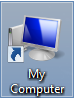
\includegraphics[width=\textwidth]{./Manual/Installation/MyComputer.png}
    \caption{Open 'My Computer'}
\end{figure}

The user will then need to right click the CD-R, and click open.

\begin{figure}[H]
    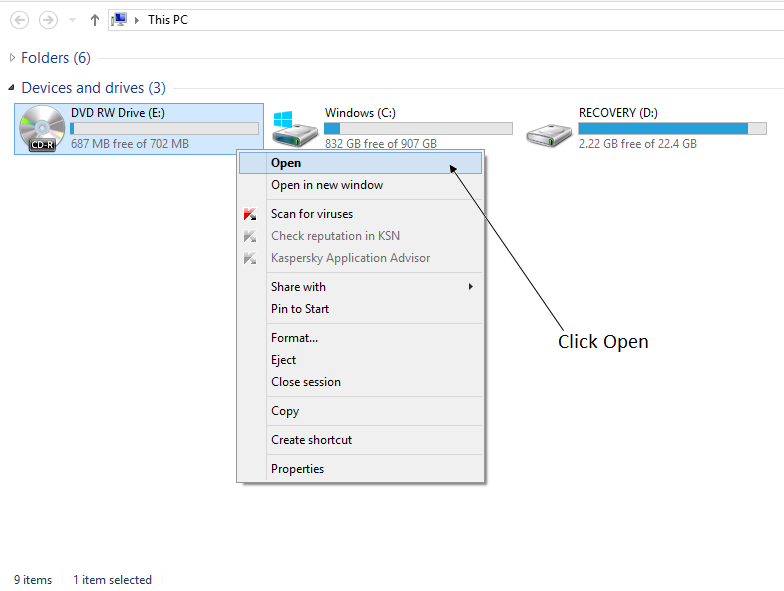
\includegraphics[width=\textwidth]{./Manual/Installation/OpenCDR.png}
    \caption{Opening the CD-R}
\end{figure}

Then right click on the installation file, and click 'Install'.

\begin{figure}[H]
    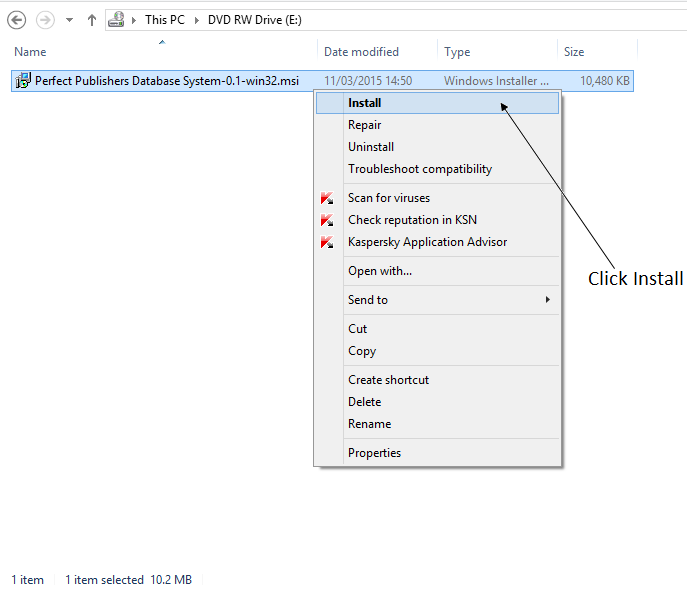
\includegraphics[width=\textwidth]{./Manual/Installation/Install.png}
    \caption{Clicking 'Install'}
\end{figure}

The Windows installer will the commence installing. The user is required to select a destination to be installed at, with the default directory given.

\begin{figure}[H]
    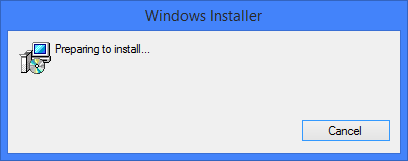
\includegraphics[width=\textwidth]{./Manual/Installation/PrepareInstall.png}
    \caption{Installing begins}
\end{figure}

\begin{figure}[H]
    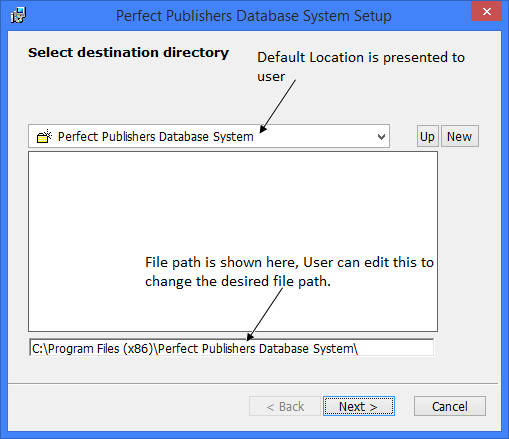
\includegraphics[width=\textwidth]{./Manual/Installation/Setup.png}
    \caption{Setup Screen}
\end{figure}

\begin{figure}[H]
    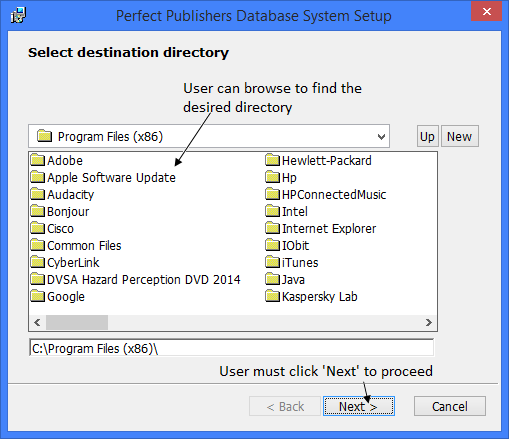
\includegraphics[width=\textwidth]{./Manual/Installation/Setup2.png}
    \caption{Setup Screen Browsing}
\end{figure}

The Installer initialises the screen for installation.

\begin{figure}[H]
    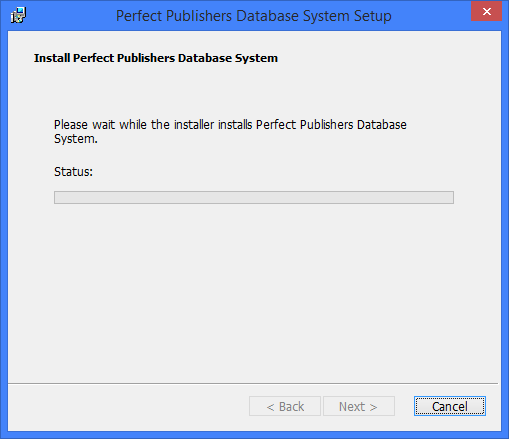
\includegraphics[width=\textwidth]{./Manual/Installation/PleaseWaitScreen.png}
    \caption{'Please Wait' Screen}
\end{figure}

The user must grant the installer permission to complete installation. To do so, click 'Yes' when the prompt opens.

\begin{figure}[H]
    
\includegraphics[width=\textwidth]{./Manual/Installation/Permission.png}
    \caption{Prompt for permission}
\end{figure}

Once the user has granted the installer permission, the installation is completed.

\begin{figure}[H]
    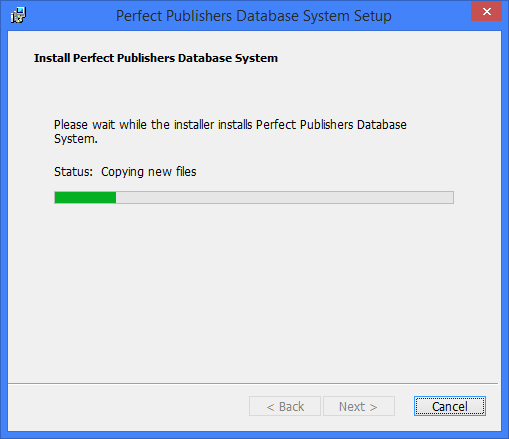
\includegraphics[width=\textwidth]{./Manual/Installation/Installing.png}
    \caption{Installation process}
\end{figure}

\begin{figure}[H]
    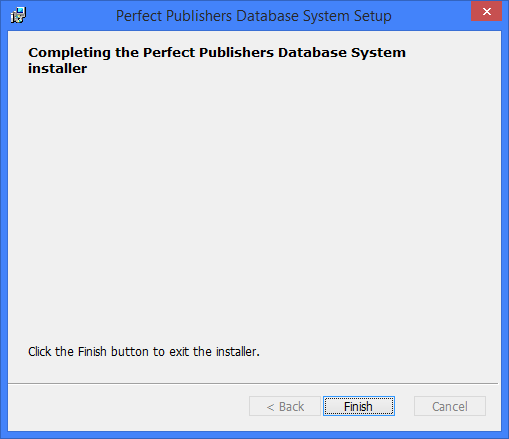
\includegraphics[width=\textwidth]{./Manual/Installation/Installed.png}
    \caption{Finished Installing}
\end{figure}


\subsection{Running the System}

In order to run the system, the user could navigate to the path of installation, or the user could create a shortcut to run quickly.

To create a shortcut, the user must do the following:

\begin{figure}[H]
    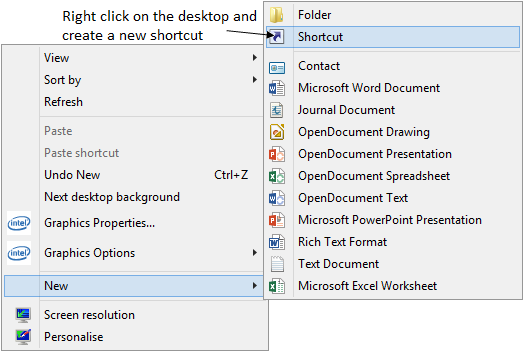
\includegraphics[width=\textwidth]{./Manual/Installation/Shortcut.png}
    \caption{Creating a shortcut}
\end{figure}

\begin{figure}[H]
    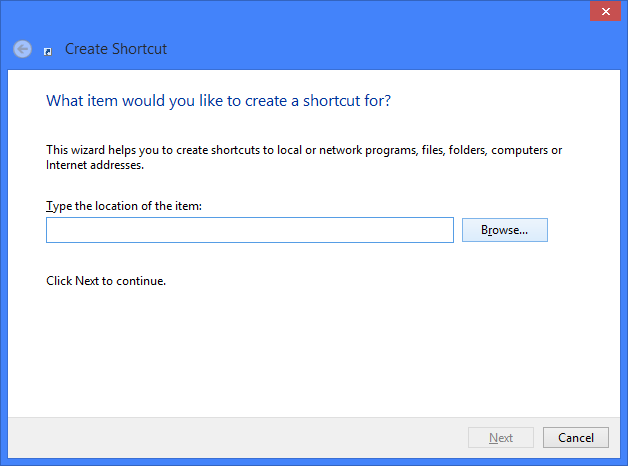
\includegraphics[width=\textwidth]{./Manual/Installation/CreateShortcut.png}
    \caption{Create shortcut screen}
\end{figure}

The user will be presented with the interface to type the file path of the system file. The user should click 'Browse...', where the user should browse to the correct file shown in Figure \ref{fig:BrowseFile}.

\begin{figure}[H]
    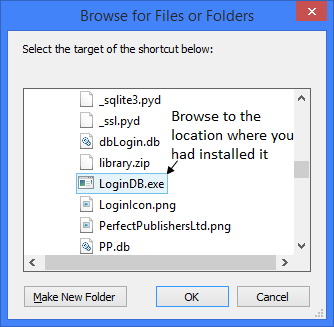
\includegraphics[width=\textwidth]{./Manual/Installation/BrowseFile.png}
    \caption{File Browsing} \label{fig:BrowseFile}
\end{figure}

\begin{figure}[H]
    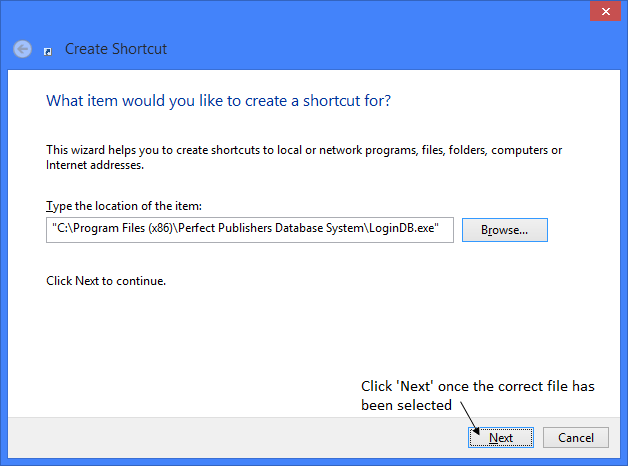
\includegraphics[width=\textwidth]{./Manual/Installation/FileSelected.png}
    \caption{File Selected} \label{fig:FileSelected}
\end{figure}


Then the user is required to name the shortcut. Afterwards, the user needs to click finish to finish creating a shortcut that the program can be run from.

\begin{figure}[H]
    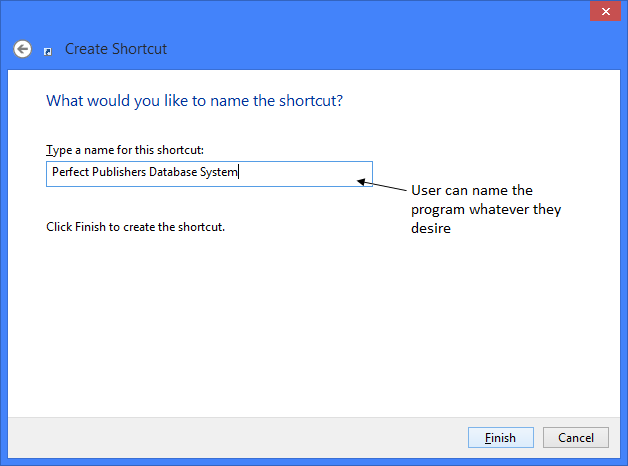
\includegraphics[width=\textwidth]{./Manual/Installation/NameShortcut.png}
    \caption{Naming shortcut}
\end{figure}

\section{Tutorial}

\subsection{Introduction}

In this section I will go through the steps of using the system to its full capabilities, including adding, editing and deleting data in the database, conducting calculations to find costs and payment prices, and searching for data in the database. I will also cover the navigation of the program.

\subsection{Assumptions}

I expect that the user has at least a basic understanding of Windows 7/8. As my client is capable with using these operating systems, the tutorial should not be difficult to follow. Also, for functions in the system that have similar functionality, only one of these functions will be properly investigated in my tutorial. For example, I will cover how to search for a book, and in doing so, I can assume that the user will be able to conduct searches for Royalties/Invoices etc., because of the similar functionality.

\subsection{Tutorial Questions}

The following sections will show how to use different parts of the system, step by step. I have simplified these down into Questions, which i have answered using these step by step tutorials. These can be referenced in the following table.

\begin{center}
\begin{tabular}{|p{3cm}|p{3cm}|p{3cm}|}
        \hline
        \textbf{Section Number} & \textbf{Question} & \textbf{Page Number} \\ \hline
        1 & "How do I add a customer?" & \pageref{sssec:Q1} \\ \hline
        2 & "How do I update customer details?" & \pageref{sssec:Q2} \\ \hline
        3 & "How do I delete a customer?" & \pageref{sssec:Q3} \\ \hline
        4 & "How do I view a customer's books?" & \pageref{sssec:Q4} \\ \hline
        5 & "How do I add a customer's book?" & \pageref{sssec:Q5} \\ \hline
        6 & "How do I update a customer's book?" & \pageref{sssec:Q6} \\ \hline
        7 & "How do I delete a customer's book?" & \pageref{sssec:Q7} \\ \hline
        8 & "How do I view customers' publishing invoices?" & \pageref{sssec:Q8} \\ \hline
        9 & "How do I view customers' book invoice items of a book?" & \pageref{sssec:Q9} \\ \hline
        10 & "How do I view customers' royalty items of a book?" & \pageref{sssec:Q10} \\ \hline
        11 & "How do I calculate a book invoice payment?" & \pageref{sssec:Q11} \\ \hline
        12 & "How do I calculate a royalty payment?" & \pageref{sssec:Q12} \\ \hline
        13 & "How do I search for an author?" & \pageref{sssec:Q13} \\ \hline
        14 & "How do I search for an author's book?" & \pageref{sssec:Q14} \\ \hline
        15 & "How do I change my Username/Password?" & \pageref{sssec:Q15} \\ \hline
\end{tabular}
\end{center}

%include as many subsubsections as necessary for each question in your list
\subsubsection{1 - How do I add a customer?} \label{sssec:Q1}

1. On the Main Menu, click on the 'Add Entry' button. A window to add a customer entry is diplayed.

\begin{figure}[H]
    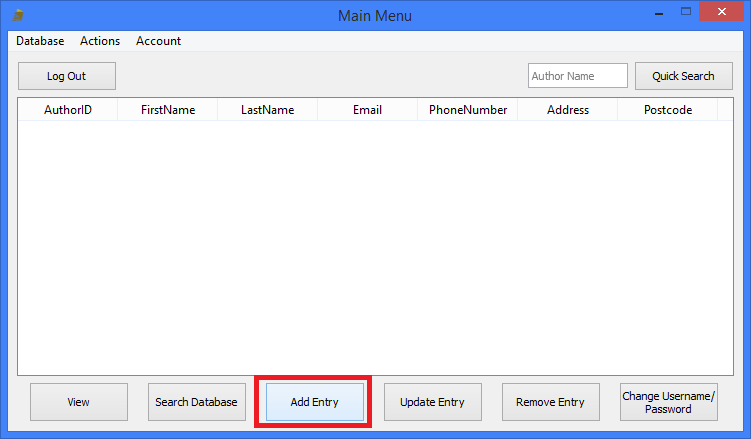
\includegraphics[width=\textwidth]{./Manual/Tutorial/Q1/AddEntryHighlighted.png}
\end{figure}


2. Fill in each box of the table with the appropriate data. Then click "Confirm".

\begin{figure}[H]
    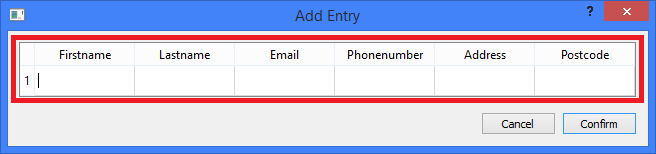
\includegraphics[width=\textwidth]{./Manual/Tutorial/Q1/AddingEntry.png}
\end{figure}

3. After clicking "Confirm", the data will be validated, then added to the system if valid.

\subsubsection{2 -  How do I update customer details?} \label{sssec:Q2}

1. On the Main Menu, choose a customer, and click on him/her. Then click "Update Entry".

\begin{figure}[H]
    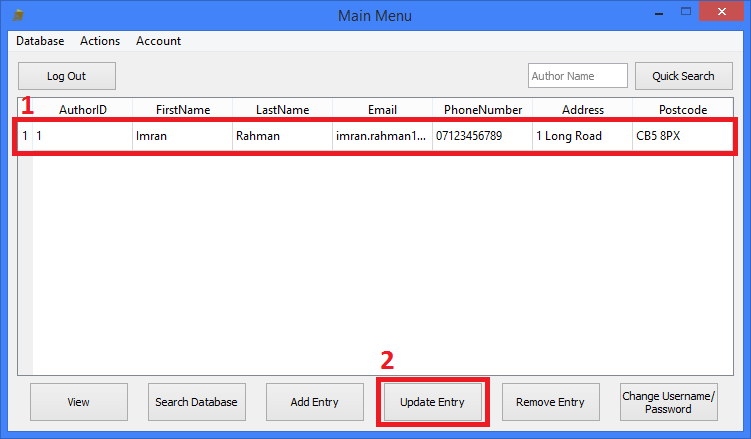
\includegraphics[width=\textwidth]{./Manual/Tutorial/Q2/SelectingEntry.png}
\end{figure}

2. A window to update the selected customer entry is displayed. To edit a field, select one, then click "Edit".

\begin{figure}[H]
    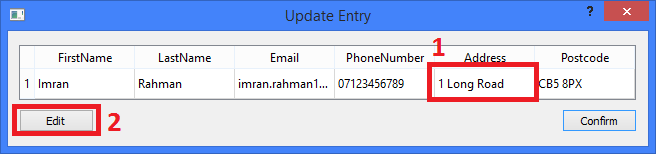
\includegraphics[width=\textwidth]{./Manual/Tutorial/Q2/EditField.png}
\end{figure}

3. Upon clicking edit, a window opens, prompting for a new entry for that field. After clicking "Confirm", the change is temporarily made, and more fields can be edited. Once finished, click "Confirm" to save changes. 

\begin{figure}[H]
    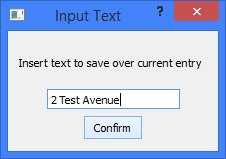
\includegraphics[width=\textwidth]{./Manual/Tutorial/Q2/InputText.png}
\end{figure}

\begin{figure}[H]
    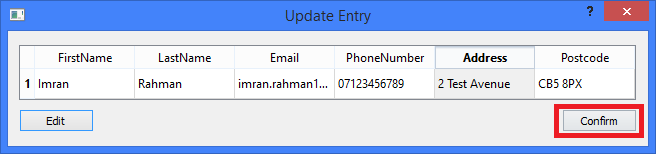
\includegraphics[width=\textwidth]{./Manual/Tutorial/Q2/Confirm.png}
\end{figure}

4. A window is displayed, asking for the password. Once the correct password has been entered and the user clicks "Confirm", the changes are saved to the database.

\begin{figure}[H]
    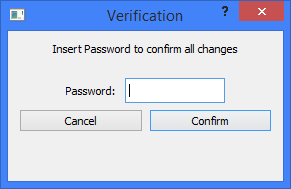
\includegraphics[width=\textwidth]{./Manual/Tutorial/Q2/Verification.png}
\end{figure}

\subsubsection{3 -  How do I delete a customer?} \label{sssec:Q3}

1. On the Main Menu, choose a customer, and click on him/her. Then click "Remove Entry".

\begin{figure}[H]
    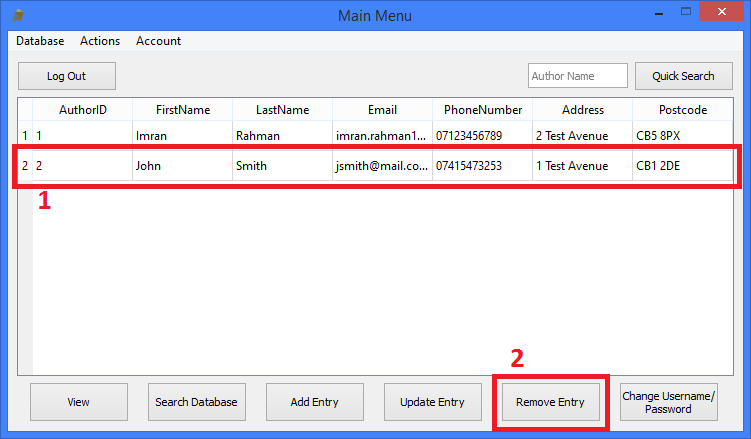
\includegraphics[width=\textwidth]{./Manual/Tutorial/Q3/SelectingCustomer.png}
\end{figure}

2. A window is displayed, asking for the password to confirm the deletion of the customer and all of their data. Once the correct password has been entered, click "Confirm". The deletion is then completed.

\begin{figure}[H]
    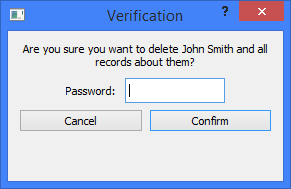
\includegraphics[width=\textwidth]{./Manual/Tutorial/Q3/Verification.png}
\end{figure}

\begin{figure}[H]
    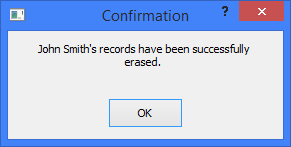
\includegraphics[width=\textwidth]{./Manual/Tutorial/Q3/Erased.png}
\end{figure}

\subsubsection{4 -  How do I view a customer's books?} \label{sssec:Q4}

1. On the Main Menu, choose a customer, and click on him/her. Then click "View".

\begin{figure}[H]
    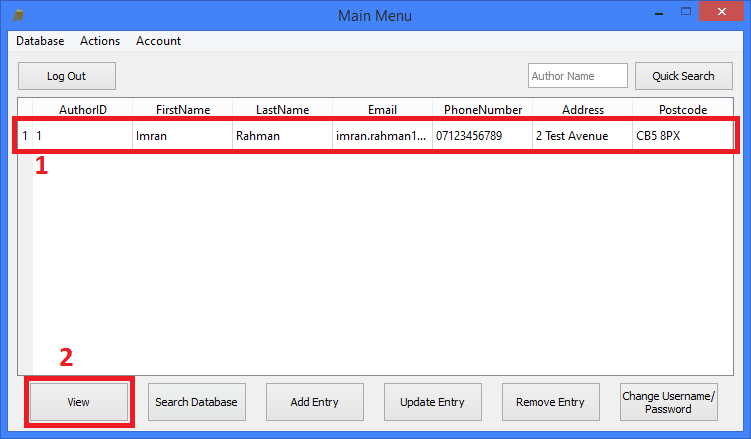
\includegraphics[width=\textwidth]{./Manual/Tutorial/Q4/View.png}
\end{figure}

2. A new layout for interactions with books is displayed, and a list of the books from the selected customer. 

\begin{figure}[H]
    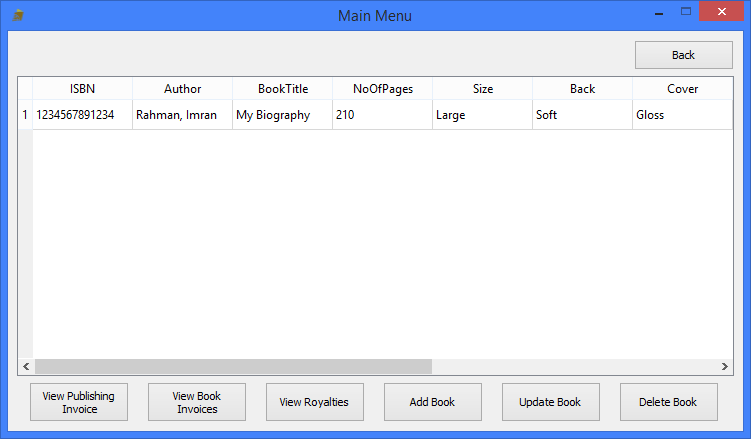
\includegraphics[width=\textwidth]{./Manual/Tutorial/Q4/CustomerBooks.png}
\end{figure}

\subsubsection{5 -  How do I add a customer's book?} \label{sssec:Q5}

1. Follow section 4 to select a customer to add books to.

2. On the Menu presenting a customer's books, click "Add Book".

\begin{figure}[H]
    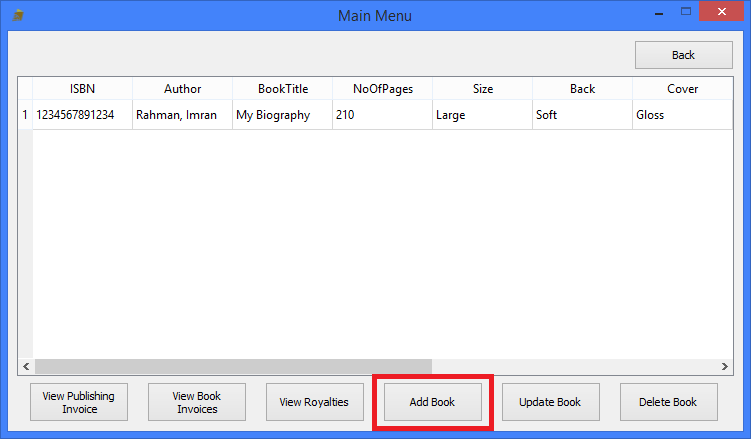
\includegraphics[width=\textwidth]{./Manual/Tutorial/Q5/AddBook.png}
\end{figure}

3. A window is opened, showing empty fields required to be filled in. After filling in the appropriate data, click "Confirm" to add the book to the database.

\begin{figure}[H]
    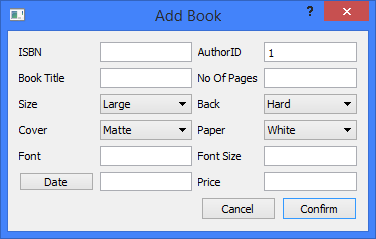
\includegraphics[width=\textwidth]{./Manual/Tutorial/Q5/AddBookWindow.png}
\end{figure}

\subsubsection{6 -  How do I update a customer's book?} \label{sssec:Q6}

1. Follow section 4 to select a customer to find their books.

2. On the Menu presenting a customer's books, choose a book, and click on it. Then click "Update Book".

\begin{figure}[H]
    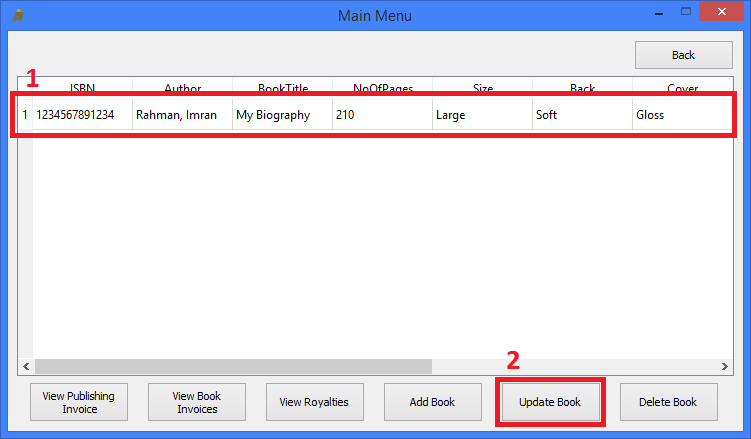
\includegraphics[width=\textwidth]{./Manual/Tutorial/Q6/UpdateBook.png}
\end{figure}

3. A window is opened, showing the current details of the book in their respective fields. All fields can be freely edited where necessary. Once finished, click "Confirm".

\begin{figure}[H]
    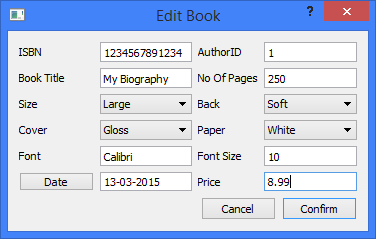
\includegraphics[width=\textwidth]{./Manual/Tutorial/Q6/EditBook.png}
\end{figure}

4. A window is displayed, asking for the password. Once the correct password has been entered and the user clicks "Confirm", the changes are saved to the database.

\begin{figure}[H]
    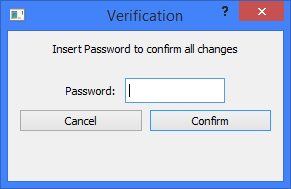
\includegraphics[width=\textwidth]{./Manual/Tutorial/Q6/Verification.png}
\end{figure}

\subsubsection{7 -  How do I delete a customer's book?} \label{sssec:Q7}

1. Follow section 4 to select a customer to find their books.

2. Click on a book entry, then click "Delete Book".

\begin{figure}[H]
    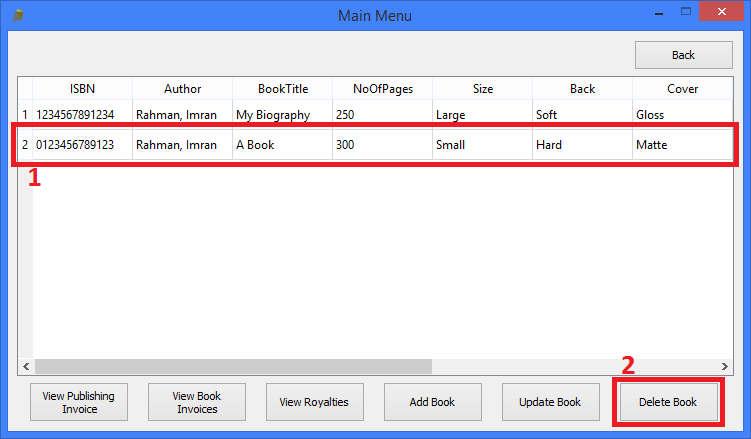
\includegraphics[width=\textwidth]{./Manual/Tutorial/Q7/DeleteBook.png}
\end{figure}

2. A window is displayed, asking for the password to confirm the deletion of the book. Once the correct password has been entered, click "Confirm". The deletion is then completed.

\begin{figure}[H]
    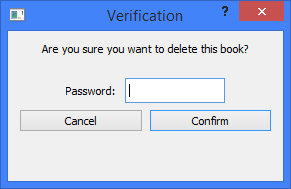
\includegraphics[width=\textwidth]{./Manual/Tutorial/Q7/Verification.png}
\end{figure}

\begin{figure}[H]
    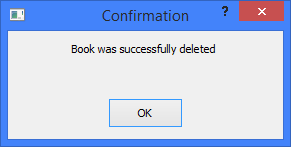
\includegraphics[width=\textwidth]{./Manual/Tutorial/Q7/Deleted.png}
\end{figure}

\subsubsection{8 -  How do I view a customers' publishing invoices?} \label{sssec:Q8}

1. Follow section 4 to select a customer to find their books.

2. Click on a book entry, then click "View Publishing Invoice".

\begin{figure}[H]
    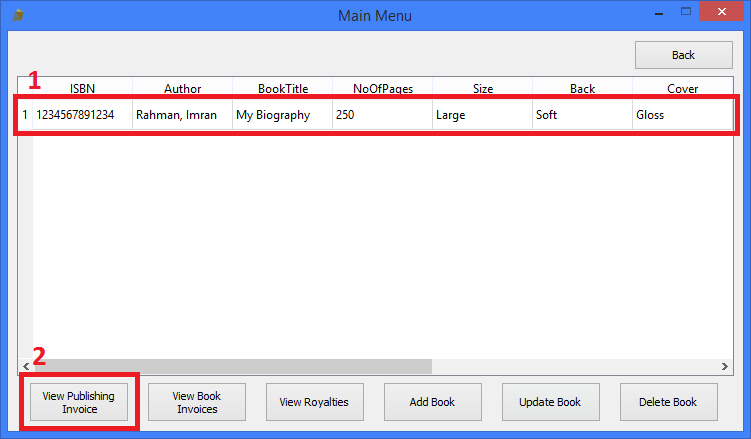
\includegraphics[width=\textwidth]{./Manual/Tutorial/Q8/ViewPubInvoice.png}
\end{figure}

3. The selected book's publishing invoice(s) is displayed.

\begin{figure}[H]
    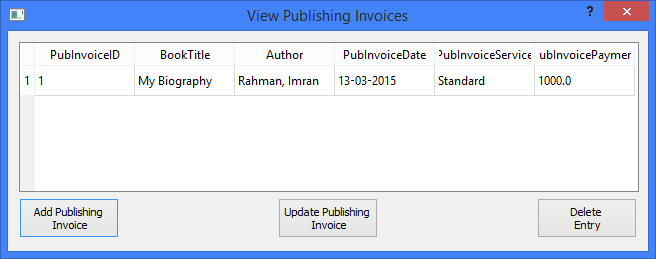
\includegraphics[width=\textwidth]{./Manual/Tutorial/Q8/PubInvoices.png}
\end{figure}

\subsubsection{9 -  How do I view customers' book invoice items of a book?} \label{sssec:Q9}

1. Follow section 4 to select a customer to find their books.

2. Click on a book entry, then click "View Book Invoices".

\begin{figure}[H]
    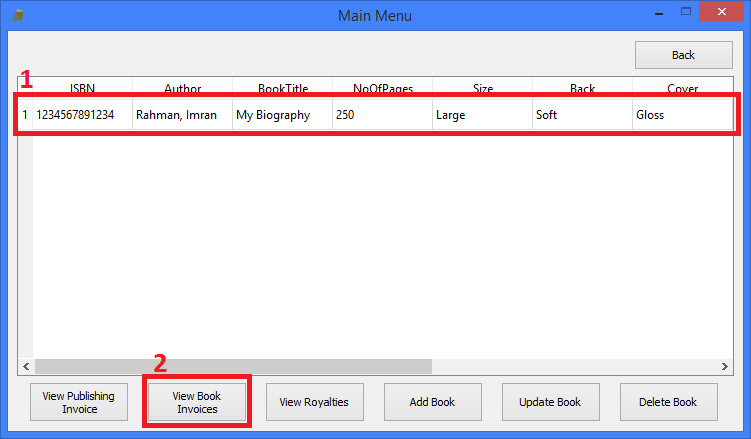
\includegraphics[width=\textwidth]{./Manual/Tutorial/Q9/ViewBookInvoices.png}
\end{figure}

3. Click on a book invoice, then click "View Book Invoice Items".

\begin{figure}[H]
    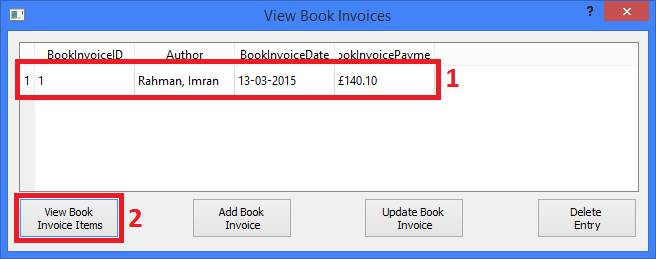
\includegraphics[width=\textwidth]{./Manual/Tutorial/Q9/ViewBookInvoiceItems.png}
\end{figure}

4. The items of the selected invoice are displayed.

\subsubsection{10 -  How do I view customers' royalty items of a book?} \label{sssec:Q10}

1. Follow section 4 to select a customer to find their books.

2. Click on a book entry, then click "View Royalties".

\begin{figure}[H]
    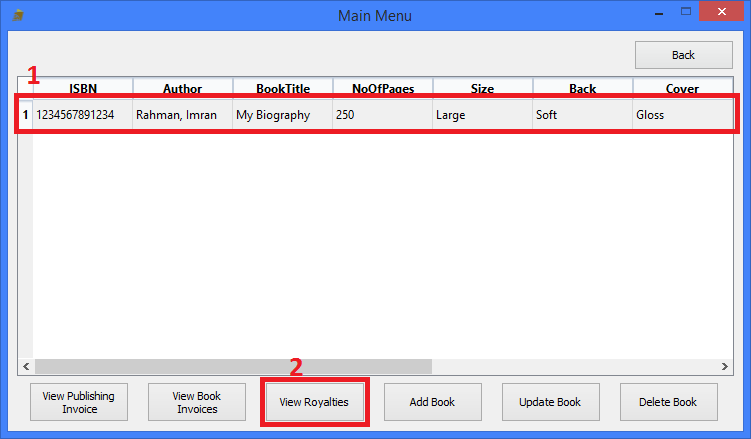
\includegraphics[width=\textwidth]{./Manual/Tutorial/Q10/ViewRoyalties.png}
\end{figure}

3. Click on a book invoice, then click "View Royalty Items".

\begin{figure}[H]
    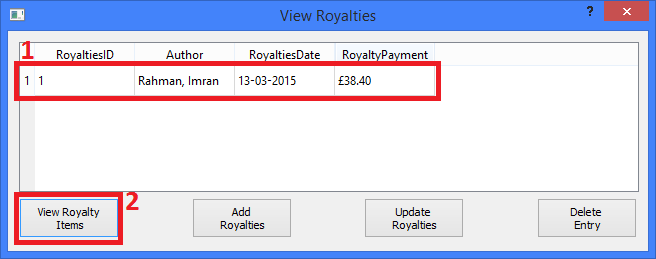
\includegraphics[width=\textwidth]{./Manual/Tutorial/Q10/ViewRoyaltyItems.png}
\end{figure}

4. The items of the selected royalty payment are displayed.

\subsubsection{11 - How do I calculate a book invoice payment?} \label{sssec:Q11}

1. Follow section 9 to navigate to a customer's book invoice items.

2. Click "Calculate" in the bottom left corner, to conduct a calculation to add to the database.

\begin{figure}[H]
    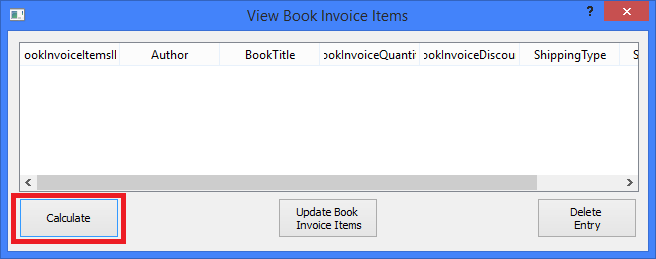
\includegraphics[width=\textwidth]{./Manual/Tutorial/Q11/CalculatePayment.png}
\end{figure}

3. Fill in the empty fields, then click "Calculate" in the bottom left corner. Afterwards, click "Confirm". This calculation will be added to the current book invoice payment and can be seen in the book invoice table.

\subsubsection{12 - How do I calculate a royalty payment?} \label{sssec:Q12}

1. Follow section 10 to navigate to a customer's royalty items.

2. Click "Calculate" in the bottom left corner, to conduct a calculation to add to the database.

\begin{figure}[H]
    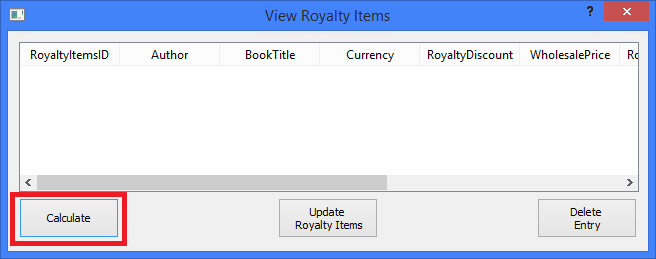
\includegraphics[width=\textwidth]{./Manual/Tutorial/Q12/CalculatePayment.png}
\end{figure}

3. Fill in the empty fields, then click "Calculate" in the bottom left corner. Afterwards, click "Confirm". This calculation will be added to the current royalty payment and can be seen in the royalties table.

\subsubsection{13 - How do I search for an author?} \label{sssec:Q13}

There are two ways to search for an author. The first way is recommended.

First method:

1. On the Main Menu, type in a customer's firstname, lastname, or both in the quick search bar in the top right corner, then click "Quick Search".

\begin{figure}[H]
    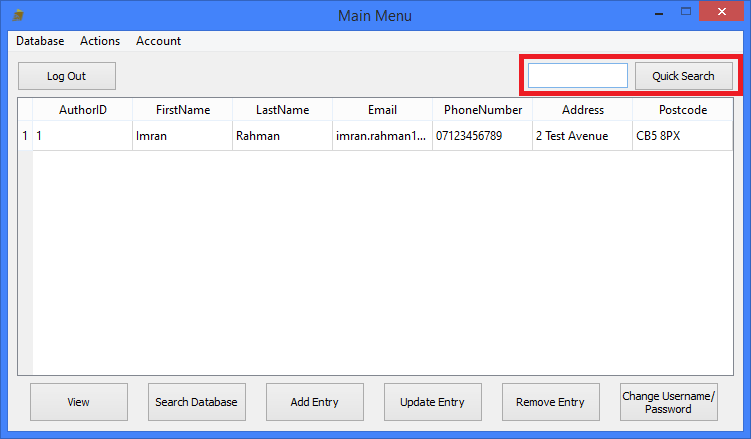
\includegraphics[width=\textwidth]{./Manual/Tutorial/Q13/QuickSearch.png}
\end{figure}

2. The results are displayed in the main window table.

Second method:

1. Click "Search Database" on the Main Menu.

\begin{figure}[H]
    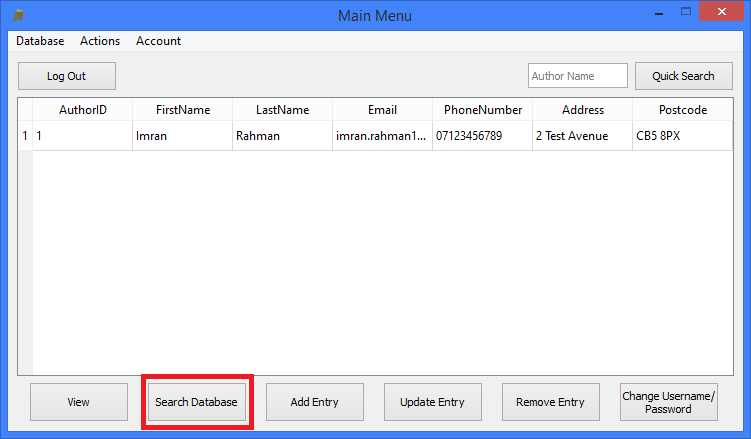
\includegraphics[width=\textwidth]{./Manual/Tutorial/Q13/SearchDatabase.png}
\end{figure}

2. A new window will open. Type in the author's first and last names in their respective boxes, and select "Author" in the first combo box. Leave the last combo box blank. Click "Search".

\begin{figure}[H]
    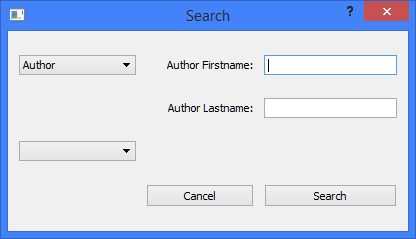
\includegraphics[width=\textwidth]{./Manual/Tutorial/Q13/SearchDatabaseWindow.png}
\end{figure}

3. The results are displayed in the main window table.

\subsubsection{14 - How do I search for an author's book?} \label{sssec:Q14}

1. Click "Search Database" on the Main Menu.

\begin{figure}[H]
    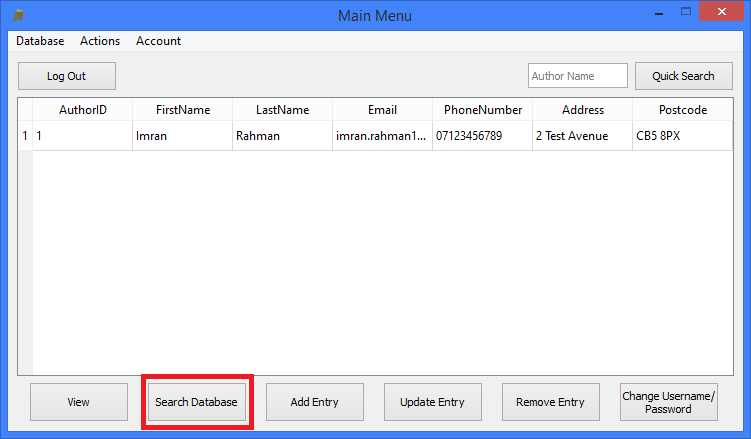
\includegraphics[width=\textwidth]{./Manual/Tutorial/Q13/SearchDatabase.png}
\end{figure}

2. Select "Book" from the first combo box.

\begin{figure}[H]
    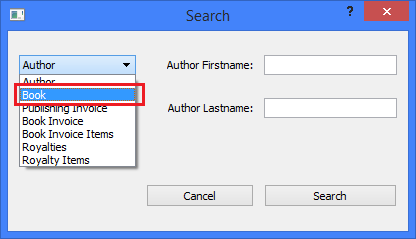
\includegraphics[width=\textwidth]{./Manual/Tutorial/Q14/BookComboBox.png}
\end{figure}

3. Select a category of the book you wish to search for from the second combo box, and then fill in the empty line edit opposite. (If a date category was selected, a date button will appear. Click it to open the calendar and select a date from it.)

\begin{figure}[H]
    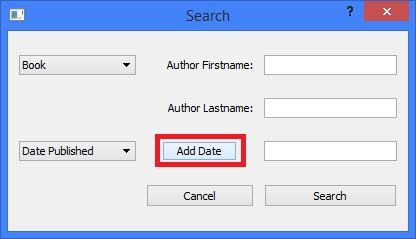
\includegraphics[width=\textwidth]{./Manual/Tutorial/Q14/DateSearch.png}
\end{figure}

\begin{figure}[H]
    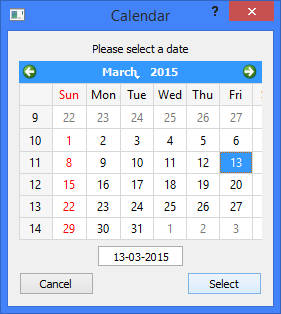
\includegraphics[width=\textwidth]{./Manual/Tutorial/Q14/SelectDate.png}
\end{figure}

4. Fill in the Firstname and Lastname boxes. Click "Search".

\begin{figure}[H]
    \includegraphics[width=\textwidth]{./Manual/Tutorial/Q14/Search.png}
\end{figure}

5. The results will be displayed in the main window table.

\subsubsection{15 - How do I change my Username/Password?} \label{sssec:Q15}

1. Click "Change Username/Password" on the Main Menu.

\begin{figure}[H]
    \includegraphics[width=\textwidth]{./Manual/Tutorial/Q15/ChangeUsernameOrPassword.png}
\end{figure}

2. If you want to change your Password, click "Change Password" and skip to step 5. Otherwise, click "Change Username".

\begin{figure}[H]
    \includegraphics[width=\textwidth]{./Manual/Tutorial/Q15/Selection.png}
\end{figure}

3. Enter your Old username in the top box, and your new username in middle box and last box for verification. Then click "Confirm".

\begin{figure}[H]
    \includegraphics[width=\textwidth]{./Manual/Tutorial/Q15/ChangeUsername.png}
\end{figure}

4. Your Username has been successfully changed.

\begin{figure}[H]
    \includegraphics[width=\textwidth]{./Manual/Tutorial/Q15/UsernameChanged.png}
\end{figure}

5. Enter your Old Password in the top box, and your new Password in middle box and last box for verification. Then click "Confirm".

\begin{figure}[H]
    \includegraphics[width=\textwidth]{./Manual/Tutorial/Q15/ChangePassword.png}
\end{figure}

6. Your Password has been successfully changed.

\begin{figure}[H]
    \includegraphics[width=\textwidth]{./Manual/Tutorial/Q15/PasswordChanged.png}
\end{figure}

\subsection{Saving}

All saving in the system is done automatically, including calculations of royalty and invoice payments. This means that no saving is requred to be manually done by the user. Data is saved after each interaction of adding, editing and deleting it, so that if there is a program crash, or the computer being used is switched off, data is not lost. However, data should only be backed up after usage of the system.

\subsection{Limitations}

My system cannot edit data upon searching for it. This was not done because I did not have enough time to implement this into the system. However, this is not difficult to create, and could be included in future versions of the system. Also, when adding customer/book data, the data is not checked against the database for duplications. This is because I did not have enough time to finish this element of the system. However, the clarity of the data in the system means that the user does not need to duplicate entries as data can easily be searched for, meaning that the user can check the existence of the data before adding it.

\section{Error Recovery}

%include as many subsections as necessary for each error
\subsection{Invalid entiries when calculating payments}

When calculating royalty/invoice payments, try to avoid entering invalid entries before calculations. This is because the window will prompt you of an invalid entry, and will then close, but still preventing the adding of the invalid data.

\begin{figure}[H]
    \includegraphics[width=\textwidth]{./Manual/InvalidEntries.png}
    \caption{Invalid Royalty Items Entries}
\end{figure}

\begin{figure}[H]
    \includegraphics[width=\textwidth]{./Manual/InvalidEntries2.png}
    \caption{Invalid Book Invoice Items Entries}
\end{figure}

\begin{figure}[H]
    \includegraphics[width=\textwidth]{./Manual/Prompt.png}
    \caption{User is prompted}
\end{figure}

In order to solve these issues, just reopen the window to calculate the payments and reenter the data.


\section{System Recovery}

\subsection{Backing-up Data}

In order to backup my program, the user will preferably need a hard copy of the backup kept off site, perhaps through the usage of a USB drive. The user should backup the database file, as this is the only data that requires being backed up.

1. First, you must navigate to where the executable file of the system is stored.

2. You must right click the "PP.db" file, and click "Copy".

\begin{figure}[H]
    \includegraphics[width=\textwidth]{./Manual/CopyDB.png}
    \caption{Copying the database file}
\end{figure}

3. Now, the user must choose where the data should be stored. Once a destination has been chosen and navigated to, create a new folder and name it "Perfect Publishers System Database".

4. Inside the folder, paste the database file.

5. You have successfully backed up the database

\subsection{Restoring Data}

In order to restore my program, the user will need to use the hardware used to back up the database.

1. Find the directory where the file was backed up to.

2. Right click on the database file, "PP.db", and click "Copy".

\begin{figure}[H]
    \includegraphics[width=\textwidth]{./Manual/CopyBackup.png}
\end{figure}

3. Navigate to where the executable file of the system is stored.

4. Inside the folder, paste the database file. It should be automatically pasted as "PP - Copy.db"

\begin{figure}[H]
    \includegraphics[width=\textwidth]{./Manual/CopiedFile.png}
\end{figure}

5. Now, you can delete the original file and rename the newly pasted file to "PP.db".

\begin{figure}[H]
    \includegraphics[width=\textwidth]{./Manual/DeleteOriginal.png}
    \caption{Deleting Original file}
\end{figure}

\begin{figure}[H]
    \includegraphics[width=\textwidth]{./Manual/Rename.png}
    \caption{Renaming the new file}
\end{figure}

6. You have successfully restored the database.

\stopcontents[chapters]